%----------------------------------------------------------------------------------------
%	PACKAGES AND OTHER DOCUMENT CONFIGURATIONS
%----------------------------------------------------------------------------------------

\documentclass{article}

\usepackage{fancyhdr} % Required for custom headers
\usepackage{lastpage} % Required to determine the last page for the footer
\usepackage{extramarks} % Required for headers and footers
\usepackage[usenames,dvipsnames]{color} % Required for custom colors
\usepackage{graphicx} % Required to insert images
\usepackage{listings} % Required for insertion of code
\usepackage{courier} % Required for the courier font
\usepackage{lipsum} % Used for inserting dummy 'Lorem ipsum' text into the template
\usepackage{parskip}
% Margins
\topmargin=-0.45in
\evensidemargin=0in
\oddsidemargin=0in
\textwidth=6.5in
\textheight=9.0in
\headsep=0.25in
\definecolor{mygreen}{rgb}{0,0.51, 0}
\linespread{1.1} % Line spacing

% Set up the header and footer
\pagestyle{fancy}
\chead{} % Top left header
\lhead{\hmwkClass\  \hmwkTitle} % Top center head
\rhead{} % Top right header
\lfoot{\lastxmark} % Bottom left footer
\cfoot{} % Bottom center footer
\rfoot{Page\ \thepage\ of\ \protect\pageref{LastPage}} % Bottom right footer
\renewcommand\headrulewidth{0.4pt} % Size of the header rule
\renewcommand\footrulewidth{0.4pt} % Size of the footer rule

\setlength\parindent{0pt} % Removes all indentation from paragraphs

%----------------------------------------------------------------------------------------
%	CODE INCLUSION CONFIGURATION
%----------------------------------------------------------------------------------------

% \definecolor{MyDarkGreen}{rgb}{0.0,0.4,0.0} % This is the color used for comments
\lstloadlanguages{C} % Load C syntax for listings, for a list of other languages supported see: ftp://ftp.tex.ac.uk/tex-archive/macros/latex/contrib/listings/listings.pdf
\lstset{commentstyle=\color{mygreen},basicstyle=\ttfamily\scriptsize,language=C,frame=single,keywordstyle=[1]\color{Blue}\bf} % Use C in this example      



\newcommand{\csnippet}[2]{
\begin{itemize}
\item[]\lstinputlisting[caption=#2,label=#1]{#1.c}
\end{itemize}
}

%----------------------------------------------------------------------------------------
%	DOCUMENT STRUCTURE COMMANDS
%----------------------------------------------------------------------------------------

% Header and footer for when a page split occurs within a problem environment
\newcommand{\enterProblemHeader}[1]{
\nobreak\extramarks{#1}{#1 continued on next page\ldots}\nobreak
\nobreak\extramarks{#1 (continued)}{#1 continued on next page\ldots}\nobreak
}

% Header and footer for when a page split occurs between problem environments
\newcommand{\exitProblemHeader}[1]{
\nobreak\extramarks{#1 (continued)}{#1 continued on next page\ldots}\nobreak
\nobreak\extramarks{#1}{}\nobreak
}

\setcounter{secnumdepth}{0} % Removes default section numbers
\newcounter{homeworkProblemCounter} % Creates a counter to keep track of the number of problems

\newcommand{\homeworkProblemName}{}
\newenvironment{homeworkProblem}[1][Problem \arabic{homeworkProblemCounter}]{ % Makes a new environment called homeworkProblem which takes 1 argument (custom name) but the default is "Problem #"
\stepcounter{homeworkProblemCounter} % Increase counter for number of problems
\renewcommand{\homeworkProblemName}{#1} % Assign \homeworkProblemName the name of the problem
\section{\homeworkProblemName} % Make a section in the document with the custom problem count
\enterProblemHeader{\homeworkProblemName} % Header and footer within the environment
}{
\exitProblemHeader{\homeworkProblemName} % Header and footer after the environment
}

\newcommand{\problemAnswer}[1]{ % Defines the problem answer command with the content as the only argument
\noindent\framebox[\columnwidth][c]{\begin{minipage}{0.98\columnwidth}#1\end{minipage}} % Makes the box around the problem answer and puts the content inside
}

\newcommand{\homeworkSectionName}{}
\newenvironment{homeworkSection}[1]{ % New environment for sections within homework problems, takes 1 argument - the name of the section
\renewcommand{\homeworkSectionName}{#1} % Assign \homeworkSectionName to the name of the section from the environment argument
\subsection{\homeworkSectionName} % Make a subsection with the custom name of the subsection
\enterProblemHeader{\homeworkProblemName\ [\homeworkSectionName]} % Header and footer within the environment
}{
\enterProblemHeader{\homeworkProblemName} % Header and footer after the environment
}

%----------------------------------------------------------------------------------------
%	NAME AND CLASS SECTION
%----------------------------------------------------------------------------------------

\newcommand{\hmwkTitle}{Assignment\ \#3} % assignment title
\newcommand{\hmwkDueDate}{Monday,\ December\ 1,\ 2014} % due date
\newcommand{\hmwkClass}{Programming Concurrent Systems} % class
\newcommand{\hmwkClassTime}{} % lecture time
\newcommand{\hmwkClassInstructor}{} % lecturer
\newcommand{\hmwkAuthorName}{Alyssa - Ilias} %name

%----------------------------------------------------------------------------------------
%	TITLE PAGE
%----------------------------------------------------------------------------------------

\title{
\vspace{2in}
\textmd{\textbf{\hmwkClass:\ \hmwkTitle}}\\
\normalsize\vspace{0.1in}\small{Due\ on\ \hmwkDueDate}\\
\vspace{0.1in}\large{\textit{\hmwkClassInstructor\ \hmwkClassTime}}
\vspace{3in}
}

\author{\textbf{\hmwkAuthorName}}


%----------------------------------------------------------------------------------------

\begin{document}

\maketitle

%----------------------------------------------------------------------------------------
%	TABLE OF CONTENTS
%----------------------------------------------------------------------------------------

%\setcounter{tocdepth}{1} % Uncomment this line if you don't want subsections listed in the ToC

%\newpage
%\tableofcontents
\newpage

%----------------------------------------------------------------------------------------
%	Introduction
%----------------------------------------------------------------------------------------
\begin{homeworkProblem}[Introduction]
	For this assignment, we were asked to parallelize our sequential heat dissipation implementation
	using the pthread library. Moreover, we had to experiment with the concepts of mutual exclusion,
	barriers, critical sections and semaphores. Specifically, we implemented a generic barrier which
	uses either mutex locks combined with condition variables, sempahores or the built-in posix functions.
	Also, we implemented a sorting algorithm which uses a pipeline of threads and bounded buffers. Lastly,
	we implemented a best effort generic program that shows the differences between constructs such as STM 
	and readers-writers locks. 

\end{homeworkProblem}
%----------------------------------------------------------------------------------------
%	Heat
%----------------------------------------------------------------------------------------

% To have just one problem per page, simply put a \clearpage after each problem

\begin{homeworkProblem}[Heat dissipation | pthreads]
\textbf{Solution description}

In order to achieve good performance, we implemented the solution by spawning threads only once, hence avoiding
the overhead of thread creation. In order to do that, we create the threads before anything else is done and since
we know the matrix sizes and as before the problem being embarrassingly parallelizable each thread gets assigned to a specific workspace. 
A set of rows that is. 

\csnippet{threadspwn}{Creation and work assignment of threads}

Much similar in the manner that openmp works. Also, in order to have correct results we put a barrier
between the actual computation and the reduction calculation thus separating the dependencies. This means a thread that has finished
its workspace has to wait for the other threads to finish.

\csnippet{synch}{Barrier synchronization}

The master thread is also waiting on a barrier for the computation and the
reduction calculation in order to do the final reduction. So we sync the working threads and the master thread by using barriers. If we have reached the iteration count the threads simply stop calculation but when we have the value lower than the threshold given we kill all the threads in the barrier waiting for the next iteration in an asynchronous way. Additionally, every thread keeps it's own copy of the pointer to the current \"snapshot\" of the values. *@alyssa it's late and i can't remember why we did this, just remember complaining. guess i never really understood in the end :P* 

\textbf{Evaluation - Experiments}

We run our experiments on the DAS-4 system using a normal node which has 8 physical cores.

The figures below show the effectivness of the parallelism. The experiments where made with the following parameters:

\begin{verbatim}
./heat -e 0.0 -i 2000 -k 2001
\end{verbatim}

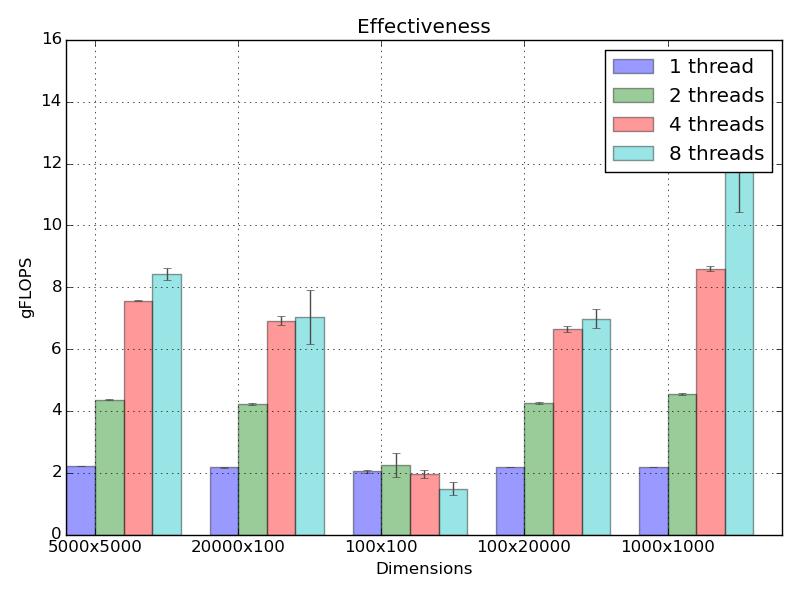
\includegraphics[width=0.75\columnwidth]{effectivness.png}

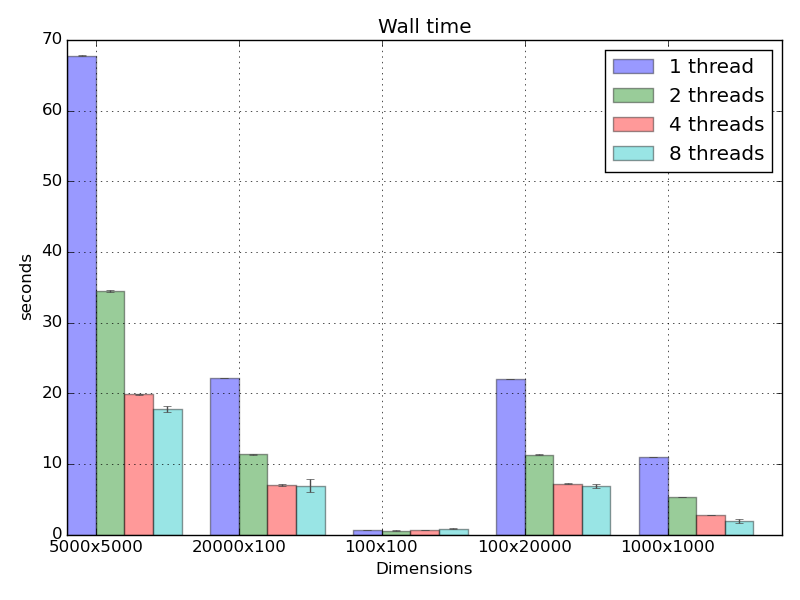
\includegraphics[width=0.75\columnwidth]{walltime.png}

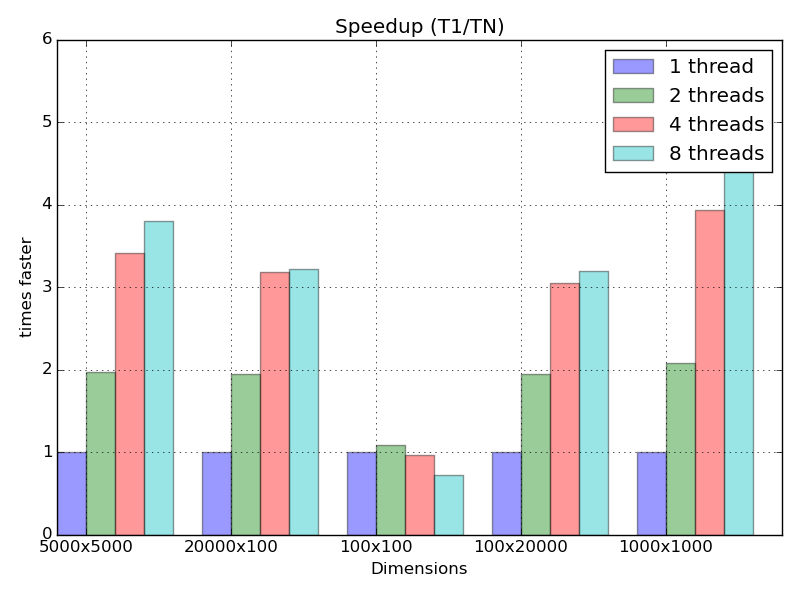
\includegraphics[width=0.75\columnwidth]{speedup.png}

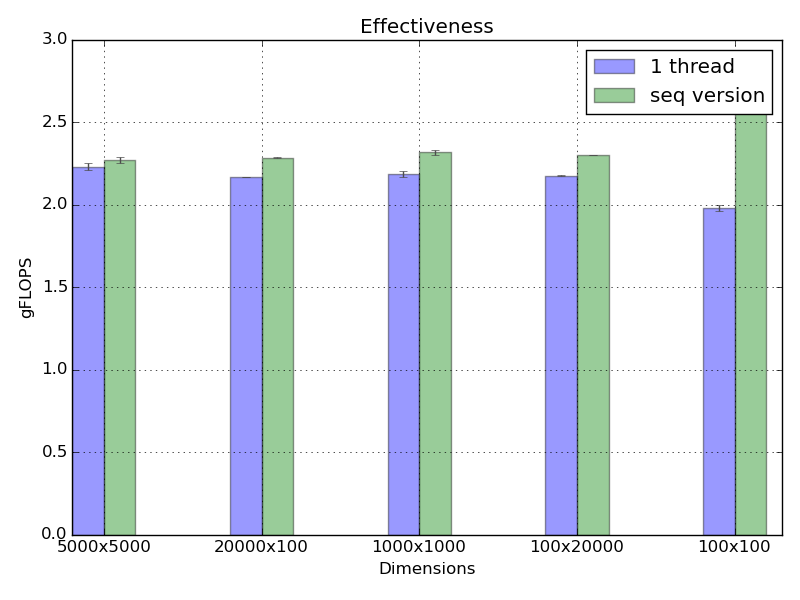
\includegraphics[width=0.75\columnwidth]{effect_seq_cmp.png}

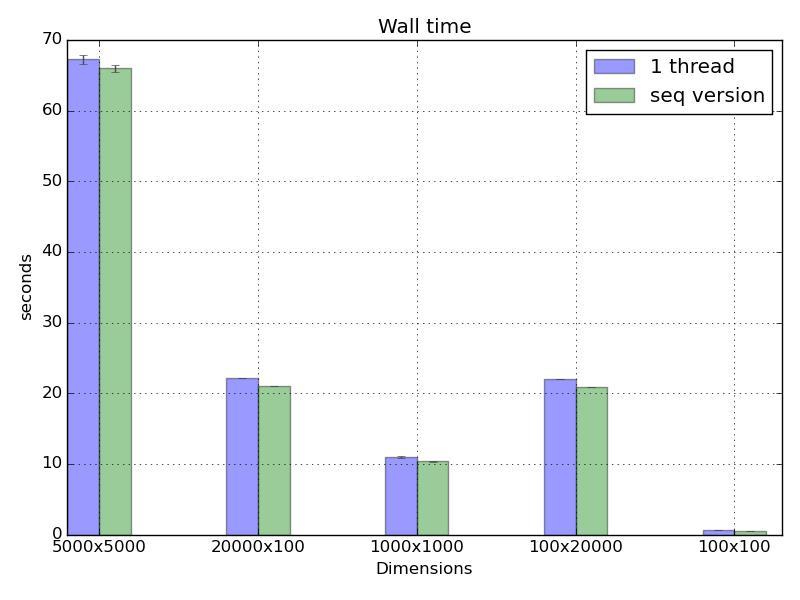
\includegraphics[width=0.75\columnwidth]{wt_seq_cmp.png}




\end{homeworkProblem}

%----------------------------------------------------------------------------------------
%	Barriers
%----------------------------------------------------------------------------------------

\begin{homeworkProblem}[Barrier synchronisation]
\textbf{Solution description}

solution desc here

\textbf{Evaluation}

experiments here

\end{homeworkProblem}

%----------------------------------------------------------------------------------------
%	Pipesort
%----------------------------------------------------------------------------------------

\begin{homeworkProblem}[Pipeline parallelism]
\textbf{Solution description}

The pipesort works as follows: The master thread creates a bounded buffer and spanws a thread associated with the buffer. After that
it generates a sequence of numbers and pushes them one by one into the buffer, thus sending them to the thread. The thread's role is 
to receive these numbers, keep the biggest value and do the same as the generator: create a new buffer plus a new thread and send the numbers
it didn't store by pushing them into the new buffer. This is done in a recursive way until the end of sequence is signaled. This occurs
by the generator sending a special symbol into the pipeline where every thread forwards it as well as its stored number to the successor. The last thread in the pipeline spawns a special thread that prints all the numbers. In the end another special symbol is forwarded which instructs the threads
to join with each other and finally end the execution. For the synchronization of the pushing and pulling from the bounded buffers we used
semaphores which are designed for this exact producer-consumer problem. Mutex locks aren't needed since for every buffer there is only a
single producer and a single consumer thus they aren't racing for particular data. Semaphores on the other hand just track the availability
of the recourses and if needed they signal blocked threads that are waiting to insert data in a full buffer or fetch data from an empty buffer.

\csnippet{sempushpull}{Semaphore handling on inserting or fetching a value}

\textbf{Evaluation}
The results are very not stable, but this is normal since a lot more threads are created than the physical cores available to handle them. This means that the scheduler plays an important role in the performance, and more importantly a role that we can't really control. In any case the following figure depicts the evaluation of the program.

%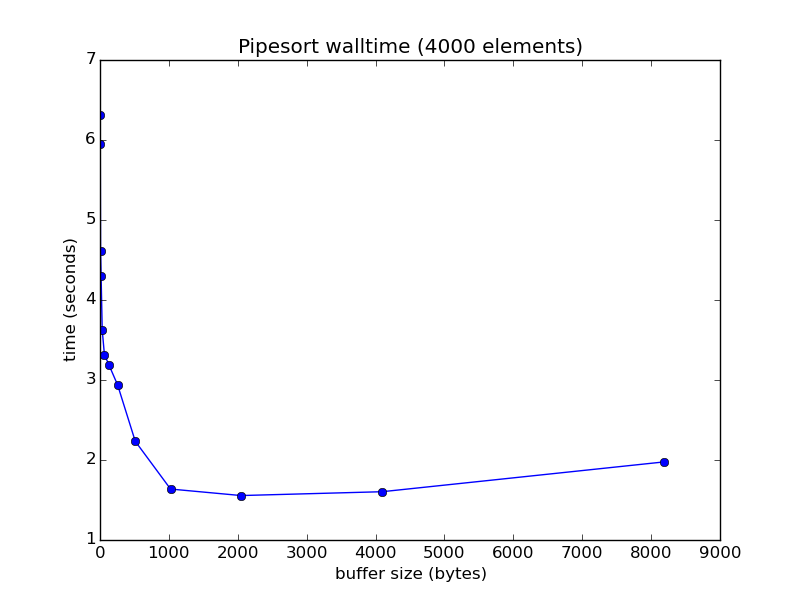
\includegraphics[width=0.75\columnwidth]{pipesort.png}

\end{homeworkProblem}

%----------------------------------------------------------------------------------------
%	critical sections
%----------------------------------------------------------------------------------------

\begin{homeworkProblem}[Mutual exclusion concepts]
\textbf{Solution description}

solution desc here

\textbf{Evaluation}

experiments here

\end{homeworkProblem}


%----------------------------------------------------------------------------------------

\end{document}
